\documentclass[a4paper, 14pt]{extarticle}

% Поля
%--------------------------------------
\usepackage{geometry}
\geometry{a4paper,tmargin=2cm,bmargin=2cm,lmargin=3cm,rmargin=1cm}
%--------------------------------------


%Russian-specific packages
%--------------------------------------
\usepackage[T2A]{fontenc}
\usepackage[utf8]{inputenc} 
\usepackage[english, main=russian]{babel}
%--------------------------------------

\usepackage{textcomp}

% Красная строка
%--------------------------------------
\usepackage{indentfirst}               
%--------------------------------------             


%Graphics
%--------------------------------------
\usepackage{graphicx}
\graphicspath{ {./images/} }
\usepackage{wrapfig}
%--------------------------------------

% Полуторный интервал
%--------------------------------------
\linespread{1.3}                    
%--------------------------------------

%Выравнивание и переносы
%--------------------------------------
% Избавляемся от переполнений
\sloppy
% Запрещаем разрыв страницы после первой строки абзаца
\clubpenalty=10000
% Запрещаем разрыв страницы после последней строки абзаца
\widowpenalty=10000
%--------------------------------------

%Списки
\usepackage{enumitem}

%Подписи
\usepackage{caption} 

%Гиперссылки
\usepackage{hyperref}

\hypersetup {
	unicode=true
}

%Рисунки
%--------------------------------------
\DeclareCaptionLabelSeparator*{emdash}{~--- }
\captionsetup[figure]{labelsep=emdash,font=onehalfspacing,position=bottom}
%--------------------------------------

\usepackage{tempora}
\usepackage{amsmath}
\usepackage{color}
\usepackage{listings}
\lstset{
  belowcaptionskip=1\baselineskip,
  breaklines=true,
  frame=L,
  xleftmargin=\parindent,
  language=Java,
  showstringspaces=false,
  basicstyle=\footnotesize\ttfamily,
  keywordstyle=\bfseries\color{blue},
  commentstyle=\itshape\color{purple},
  identifierstyle=\color{black},
  stringstyle=\color{red},
}

%--------------------------------------
%			НАЧАЛО ДОКУМЕНТА
%--------------------------------------

\begin{document}

%--------------------------------------
%			ТИТУЛЬНЫЙ ЛИСТ
%--------------------------------------
\begin{titlepage}
\thispagestyle{empty}
\newpage


%Шапка титульного листа
%--------------------------------------
\vspace*{-60pt}
\hspace{-65pt}
\begin{minipage}{0.3\textwidth}
\hspace*{-20pt}\centering

\includegraphics[width=\textwidth]{emblem}
\end{minipage}
\begin{minipage}{0.67\textwidth}\small \textbf{
\vspace*{-0.7ex}
\hspace*{-6pt}\centerline{Министерство науки и высшего образования Российской Федерации}
\vspace*{-0.7ex}
\centerline{Федеральное государственное бюджетное образовательное учреждение }
\vspace*{-0.7ex}
\centerline{высшего образования}
\vspace*{-0.7ex}
\centerline{<<Московский государственный технический университет}
\vspace*{-0.7ex}
\centerline{имени Н.Э. Баумана}
\vspace*{-0.7ex}
\centerline{(национальный исследовательский университет)>>}
\vspace*{-0.7ex}
\centerline{(МГТУ им. Н.Э. Баумана)}}
\end{minipage}
%--------------------------------------

%Полосы
%--------------------------------------
\vspace{-25pt}
\hspace{-35pt}\rule{\textwidth}{2.3pt}

\vspace*{-20.3pt}
\hspace{-35pt}\rule{\textwidth}{0.4pt}
%--------------------------------------

\vspace{1.5ex}
\hspace{-35pt} \noindent \small ФАКУЛЬТЕТ\hspace{80pt} <<Информатика и системы управления>>

\vspace*{-16pt}
\hspace{47pt}\rule{0.83\textwidth}{0.4pt}

\vspace{0.5ex}
\hspace{-35pt} \noindent \small КАФЕДРА\hspace{50pt} <<Теоретическая информатика и компьютерные технологии>>

\vspace*{-16pt}
\hspace{30pt}\rule{0.866\textwidth}{0.4pt}
  
\vspace{11em}

\begin{center}
\Large {\bf Лабораторная работа № 2} \\ 
\large {\bf по курсу <<Языки и методы программирования>>} \\ 
\large <<Разработка простейшего класса на языке Java>>
\end{center}\normalsize

\vspace{8em}


\begin{flushright}
  {Студент группы ИУ9-21Б Воронков А. С.\hspace*{15pt} \\
  \vspace{2ex}
  Преподаватель Посевин Д. П.\hspace*{15pt}}
\end{flushright}

\bigskip

\vfill
 

\begin{center}
\textsl{Москва 2026}
\end{center}
\end{titlepage}
%--------------------------------------
%		КОНЕЦ ТИТУЛЬНОГО ЛИСТА
%--------------------------------------

\renewcommand{\ttdefault}{pcr}

\setlength{\tabcolsep}{3pt}
\newpage
\setcounter{page}{2}

\section{Цель}\label{Sect::task}
\par
Изучить базовые возможности языка Java. Создать свой класс по индивидуальному варианту и "обернуть" его в веб-сервер.
\section{Персональный вариант}
Класс треугольников в трёхмерном пространстве с операцией вычисления площади.
\pagebreak
\section{Практическая реализация}
Код файла Point.java
\begin{lstlisting}
public class Point {
    private double x, y, z ;
    public Point (double x, double y, double z) {
        this.x = x;
        this.y = y;
        this.z = z;
    }

    public double getX() {return x;}
    public double getY() {return y;}
    public double getZ() {return z;}

    public String toString() {
        return String.format("(%.1f, %.1f, %.1f)", x, y, z);
    }
}
\end{lstlisting}
\par
Код файла Triangle.java
\begin{lstlisting}
    import java.lang.Math;

public class Triangle {
    private Point p1, p2, p3;
    public Triangle(Point p1, Point p2, Point p3) {
        this.p1 = p1;
        this.p2 = p2;
        this.p3 = p3;
    }

    public Point getP1() { return p1; }
    public Point getP2() { return p2; }
    public Point getP3() { return p3; }

    private double getDist(Point poi1, Point poi2) {
        return Math.sqrt(
                Math.pow(poi1.getX() - poi2.getX(), 2) +
                Math.pow(poi1.getY() - poi2.getY(), 2) +
                Math.pow(poi1.getZ() - poi2.getZ(), 2));
    }

    public double getSquare() {
        double a = getDist(p1, p2);
        double b = getDist(p2, p3);
        double c = getDist(p3, p1);
        double p = (a + b + c) / 2;
        return Math.sqrt(p * (p - a) * (p - b) * (p - c));
    }

    public String toString() {
        return "("+p1.getX()+", "+p1.getY()+", "+p1.getZ()+"),\n" +
                "("+p2.getX()+", "+p2.getY()+", "+p2.getZ()+"),\n" +
                "("+p3.getX()+", "+p3.getY()+", "+p3.getZ()+")";
    }
}
\end{lstlisting}
\par
Код файла Test.java
\begin{lstlisting}
    public class Test {
    public static void main (String [] args) {
        Point p1 = new Point(0,0, 0);
        Point p2 = new Point(30,20, 10);
        Point p3 = new Point(10,30, 40);
        Triangle trian = new Triangle(p1, p2, p3);
        System.out.println(trian);
        System.out.println("Square: " + trian.getSquare());
    }
}
\end{lstlisting}
\par
Код файла Test1.java
\begin{lstlisting}
import java.io.IOException;
import java.io.OutputStream;
import java.net.InetSocketAddress;
import java.net.URLDecoder;
import java.nio.charset.StandardCharsets;
import java.util.HashMap;
import java.util.Map;

import com.sun.net.httpserver.HttpExchange;
import com.sun.net.httpserver.HttpHandler;
import com.sun.net.httpserver.HttpServer;

class QueryParser {

  static Map<String, String> parse(String query) {
    Map<String, String> params = new HashMap<>();
    if (query == null || query.isEmpty())
      return params;

    for (String pair : query.split("&")) {
      String[] parts = pair.split("=", 2);
      if (parts.length != 2)
        continue;

      String key = URLDecoder.decode(parts[0], StandardCharsets.UTF_8);
      String value = URLDecoder.decode(parts[1], StandardCharsets.UTF_8);
      params.put(key, value);
    }
    return params;
  }
}

class TriangleMapper {

  static Triangle fromParams(Map<String, String> params) {
    double x1 = Double.parseDouble(params.getOrDefault("p1x", "0"));
    double y1 = Double.parseDouble(params.getOrDefault("p1y", "0"));
    double z1 = Double.parseDouble(params.getOrDefault("p1z", "0"));
    double x2 = Double.parseDouble(params.getOrDefault("p2x", "0"));
    double y2 = Double.parseDouble(params.getOrDefault("p2y", "0"));
    double z2 = Double.parseDouble(params.getOrDefault("p2z", "0"));
    double x3 = Double.parseDouble(params.getOrDefault("p3x", "0"));
    double y3 = Double.parseDouble(params.getOrDefault("p3y", "0"));
    double z3 = Double.parseDouble(params.getOrDefault("p3z", "0"));
    return new Triangle(new Point(x1, y1, z1),
                        new Point(x2, y2, z2),
                        new Point(x3, y3, z3));
  }
}

class TriangleJsonSerializer {

  static String toJson(Triangle t) {
    return """
        {
          "point1": %s,
          "point2": %s,
          "point3": %s,
          "square": %.2f
        }
        """.formatted(
            t.getP1().toString(),
            t.getP2().toString(),
            t.getP3().toString(),
            t.getSquare());
  }

  private static String escape(String s) {
    return s.replace("\"", "\\\"");
  }
}

public class Test1 {

  public static void main(String[] args) throws Exception {
    HttpServer server = HttpServer.create(new InetSocketAddress(5678), 0);
    server.createContext("/test", new MyHandler());
    server.setExecutor(null); // creates a default executor
    server.start();
  }

  static class MyHandler implements HttpHandler {
    @Override
    public void handle(HttpExchange exchange) throws IOException {
      if (!"GET".equals(exchange.getRequestMethod())) {
        exchange.sendResponseHeaders(405, -1);
        return;
      }

      String query = exchange.getRequestURI().getQuery();
      Map<String, String> params = QueryParser.parse(query);

      Triangle triangle;
      try {
        triangle = TriangleMapper.fromParams(params);
      } catch (NumberFormatException e) {
        exchange.sendResponseHeaders(400, -1);
        return;
      }

      String json = TriangleJsonSerializer.toJson(triangle);

      exchange.getResponseHeaders().add("Content-Type", "application/json");
      exchange.sendResponseHeaders(200, json.getBytes().length);

      try (OutputStream os = exchange.getResponseBody()) {
        os.write(json.getBytes());
      }
    }
  }
}
\end{lstlisting}

\section{Результаты}
В результате работы программы получился веб-сервер с отображением координат точек треугольника и его площади.

\begin{center}
    \nopagebreak
    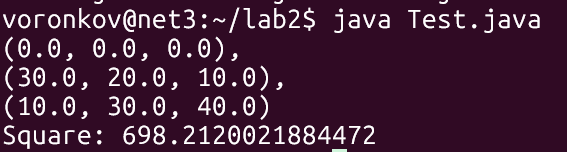
\includegraphics[width=0.85\textwidth]{test}
    \captionof{figure}{Тестирование на сервере}
    \vspace{1.5em} 

    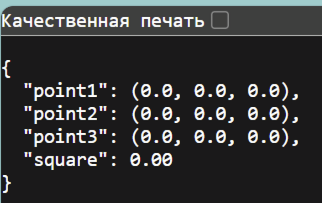
\includegraphics[width=0.85\textwidth]{empty}
    \captionof{figure}{Результат запроса http://185.102.139.168:5678/test?}
    \vspace{1.5em}

    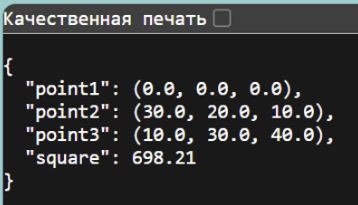
\includegraphics[width=0.85\textwidth]{web}
    \captionsetup{justification=centering}
    \captionof{figure}{Результат запроса с параметрами координат: \\ \url{http://185.102.139.168:5678/test?p1x=0&p1y=0&p1z=0&p2x=30&p2y=20&p2z=10&p3x=10&p3y=30&p3z=40}}
\end{center}

Класс треугольник принимает на вход три объекта класса Point. Класс Point принимает на вход координаты точки в трехмерном пространстве. Веб-сервер выводит координаты точек и площадь в формате JSON.

\section{Вывод}
В данной лабораторной работе был реализован класс треугольников с операцией подсчета площади. Также он был "обернут" в веб-сервер. На котором выводится основная информация: координаты точек и площадь в формате JSON.
\end{document}